\section{Entities}

% ----------------------------------------------------------------------------------------------------------
% Accumulator
% ----------------------------------------------------------------------------------------------------------

\subsection{Accumulator}

\vspace{1em}
\begin{minipage}{\linewidth}
    \centering
    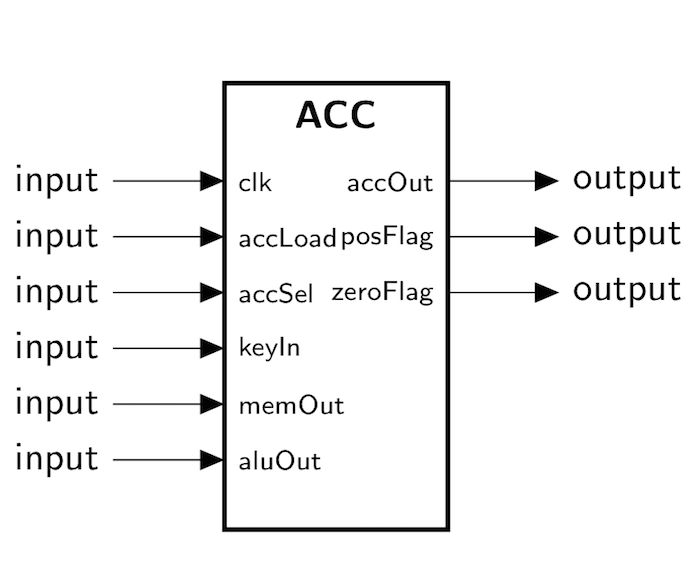
\includegraphics[width=0.4\linewidth]{images/ACC.png}
    \captionof{figure}[Accumulator Unit - Block]{Accumulator - Block}
    \label{fig:acc_block}
\end{minipage}

\subsubsection{Ports}

\vspace{1em}
\begin{table}[!h]
	\centering
	\begin{tabular}{|l|l|c|l|}
		\hline
		\textbf{Name} & \textbf{Type} & \textbf{Bitlength} & \textbf{Direction}\\
		\hline
		clk & \texttt{std\_logic} & 1 & Input \\
		\hline
		accLoad & \texttt{std\_logic} & 1 & Input \\
		\hline
		accSel & \texttt{std\_logic\_vector} & 2 & Input \\
		\hline
		keyIn & \texttt{std\_logic\_vector} & 8 & Input \\
		\hline
		memOut & \texttt{std\_logic\_vector} & 8 & Input \\
		\hline
		aluOut & \texttt{std\_logic\_vector} & 8 & Input \\
		\hline
		accOut & \texttt{std\_logic\_vector} & 8 & Output \\
		\hline
		posFlag & \texttt{std\_logic} & 1 & Output \\
		\hline
		zeroFlag & \texttt{std\_logic} & 1 & Output \\
		\hline
	\end{tabular}
	\caption{Accumulator Ports}
	\label{tab:acc_ports}
\end{table}

% ----------------------------------------------------------------------------------------------------------
% Arithmetic Logical Unit
% ----------------------------------------------------------------------------------------------------------

\pagebreak
\subsection{Arithmetic Logical Unit}

\vspace{1em}
\begin{minipage}{\linewidth}
    \centering
    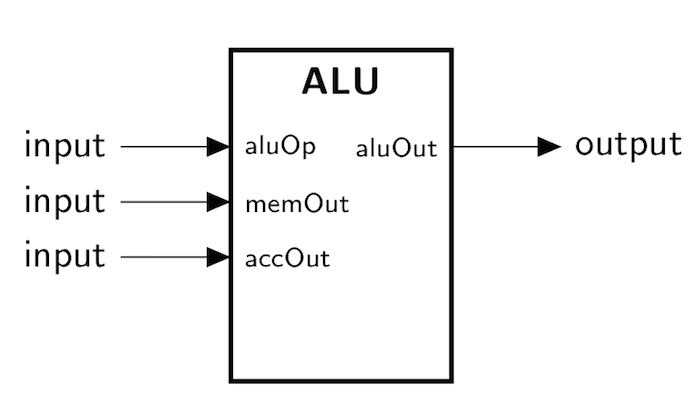
\includegraphics[width=0.4\linewidth]{images/ALU.png}
    \captionof{figure}[Arithmetic Logical Unit - Block]{Arithmetic Logical Unit - Block}
    \label{fig:alu_block}
\end{minipage}

\emph{Dies ist der einzige Baustein des HC1 ohne Taktsignal.}

\subsubsection{Ports}

\vspace{1em}
\begin{table}[!h]
	\centering
	\begin{tabular}{|l|l|c|l|}
		\hline
		\textbf{Name} & \textbf{Type} & \textbf{Bitlength} & \textbf{Direction}\\
		\hline
		aluOp & \texttt{std\_logic\_vector} & 2 & Input \\
		\hline
		memOut & \texttt{std\_logic\_vector} & 8 & Input \\
		\hline
		accOut & \texttt{std\_logic\_vector} & 8 & Input \\
		\hline
		aluOut & \texttt{std\_logic\_vector} & 8 & Output \\
		\hline
	\end{tabular}
	\caption{Arithmetic Logical Unit Ports}
	\label{tab:alu_ports}
\end{table}

% ----------------------------------------------------------------------------------------------------------
% Control Unit
% ----------------------------------------------------------------------------------------------------------

\pagebreak
\subsection{Control Unit}

\vspace{1em}
\begin{minipage}{\linewidth}
    \centering
    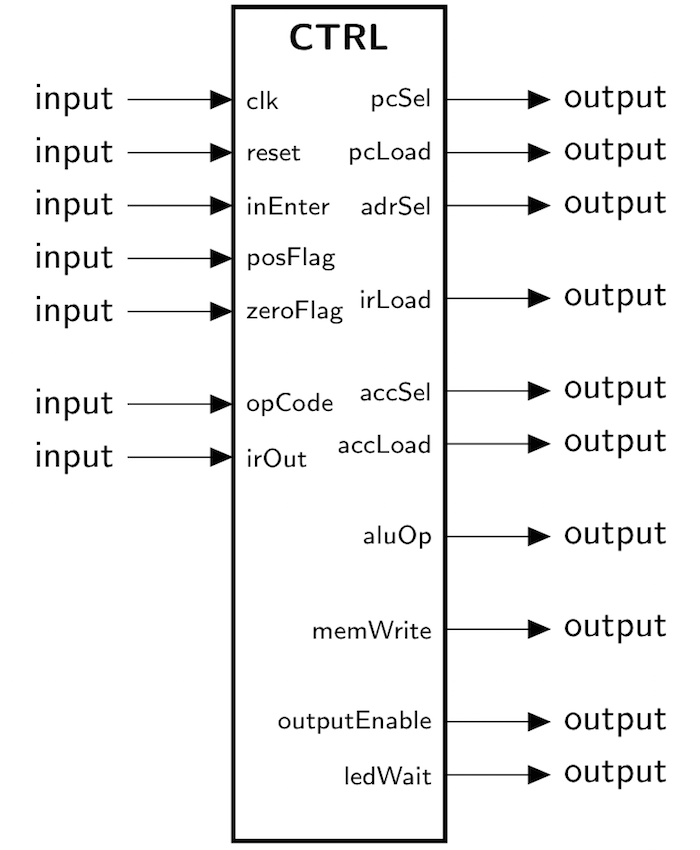
\includegraphics[width=0.4\linewidth]{images/CTRL.png}
    \captionof{figure}[Control Unit - Block]{Control Unit - Block}
    \label{fig:ctrl_block}
\end{minipage}

Die Control Unit steuert alle Prozesse des Rechners. Sie besteht aus einer State Machine welche die Eingangssignale auswertet und darauf basierend die Ausgänge setzt.

\subsubsection{Ports}

\vspace{1em}
\begin{table}[!h]
	\centering
	\begin{tabular}{|l|l|c|l|}
		\hline
		\textbf{Name} & \textbf{Type} & \textbf{Bitlength} & \textbf{Direction}\\
		\hline
		clk & \texttt{std\_logic} & 1 & Input \\
		\hline
		reset & \texttt{std\_logic} & 1 & Input \\
		\hline
		inEnter & \texttt{std\_logic} & 1 & Input \\
		\hline
		posFlag & \texttt{std\_logic} & 1 & Input \\
		\hline
		zeroFlag & \texttt{std\_logic} & 1 & Input \\
		\hline
		opCode & \texttt{std\_logic\_vector} & 3 & Input \\
		\hline
		irOut & \texttt{std\_logic\_vector} & 5 & Input \\
		\hline
	\end{tabular}
	\caption{Control Unit Input Ports}
	\label{tab:ctrl_ports_in}
\end{table}

\vspace{1em}
\begin{table}[!h]
	\centering
	\begin{tabular}{|l|l|c|l|}
		\hline
		\textbf{Name} & \textbf{Type} & \textbf{Bitlength} & \textbf{Direction}\\
		\hline
		pcSel & \texttt{std\_logic\_vector} & 1 & Output \\
		\hline
		pcLoad & \texttt{std\_logic} & 1 & Output \\
		\hline
		adrSel & \texttt{std\_logic} & 1 & Output \\
		\hline
		irLoad & \texttt{std\_logic} & 1 & Output \\
		\hline
		accSel & \texttt{std\_logic\_vector} & 2 & Output \\
		\hline
		accLoad & \texttt{std\_logic} & 1 & Output \\
		\hline
		aluOp & \texttt{std\_logic\_vector} & 2 & Output \\
		\hline
		memWrite & \texttt{std\_logic} & 1 & Output \\
		\hline
		outputEnable & \texttt{std\_logic} & 1 & Output \\
		\hline
		ledWait (optional) & \texttt{std\_logic} & 1 & Output \\
		\hline
	\end{tabular}
	\caption{Control Unit Output Ports}
	\label{tab:ctrl_ports_out}
\end{table}

Wie am Ende des Architekturkapitels \ref{modifications} erklärt ist das \emph{ledWait} Signal nicht Bestandteil des ursprünglichen HC1 Rechners.

\subsubsection{State Machine}

Im folgenden ein Beispiel wie die State Machine der Control Unit aussehen kann:

\vspace{1em}
\begin{minipage}{\linewidth}
    \centering
    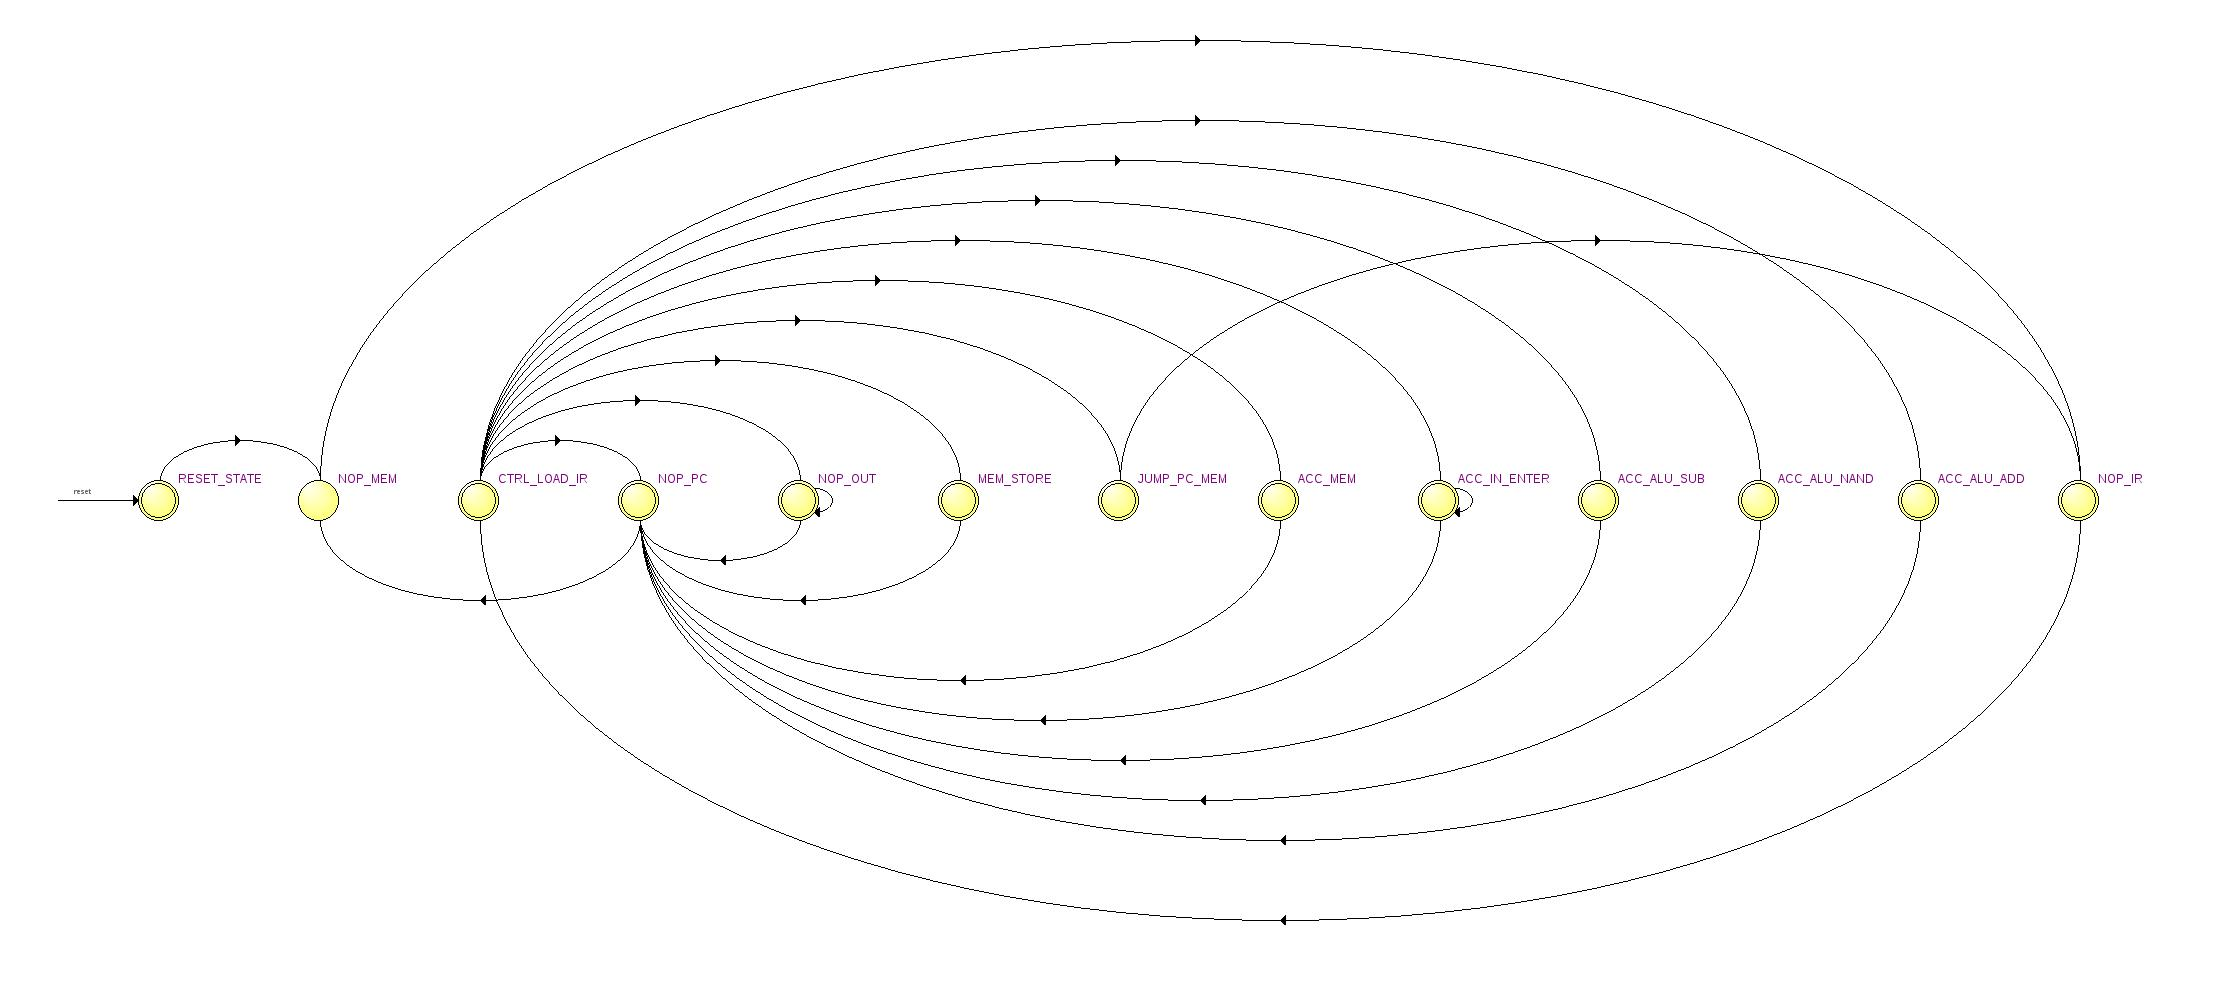
\includegraphics[width=1.0\linewidth]{images/state_machine.jpg}\\
    \captionof{figure}[Control Unit - State Machine]{Control Unit - State Machine}
    \label{fig:ctrl_state}
\end{minipage}

Da die Abbildung etwas komplex wirkt ist hier nochmals der VHDL Code zum Erstellen eines solchen State Machine Typen abgebildet.

\begin{minted}[linenos, fontsize=\footnotesize]{vhdl}
type state_type is (
        RESET_STATE,                    -- Reset CPU

        CTRL_LOAD_IR,                   -- New Instruction from IR

        MEM_STORE,                      -- Write Memory
        ACC_MEM,                        -- Acc load Memory

        ACC_ALU_ADD,                    -- Acc load ALU with ALU-Add Operation
        ACC_ALU_SUB,                    -- Acc load ALU with ALU-Sub Operation
        ACC_ALU_NAND,                   -- Acc load ALU with ALU-Nand Operation

        ACC_inEnter,                    -- Acc load key_in when inEnter is set

        JUMP_PC_MEM,                    -- PC Jump to Address in Memory

        NOP_PC,                         -- Update PC
        NOP_OUT,                        -- Enable Output while not inEnter
        NOP_MEM,                        -- Update MEM
        NOP_IR                          -- Update IR
);
\end{minted}

\subsubsection{Implementationshinweis}

Es gibt verschiedene Wege das Control Unit Verhalten in VHDL zu implementieren. Das Hauptproblem hierbei ist es einen Weg zu finden die Control Unit taktgesteuert zu impementieren ohne \emph{inferred latches} zu generieren.

Ein Weg dies zu tun ist folgender. Zuerst werden drei verschiedene Prozesse definiert:

\begin{enumerate}
	\item Eingangssignale State Prozess - \textbf{Asynchroner Prozess}
	\item Takt Prozess - \textbf{Taktsynchroner Prozess}
	\item State Ausgangssignal Prozess  - \textbf{Taktsynchroner Prozess}
\end{enumerate}

\paragraph{Eingangssignale State Prozess}

Dieser Prozess ist sensitiv gegenüber allen Eingangssignalen mit Ausnahme der \emph{clk} und des \emph{reset} Signals.

Der Prozess überprüft beim Aufrufen den aktuellen State und speichert basierend auf den Eingangssignalen den nächsten State in einem internen Signal.

\emph{Um inferred latches zu vermeiden muss der interne nächste State am Anfang des Prozesses auf den aktuellen State gesetzt werden.}

\paragraph{Takt Prozess}

Dieser Prozess aktualisiert den aktuellen State. Hierbei wird der aktuelle State durch den intern gespeicherten State überschrieben.

Zudem wird hier auch das \emph{reset} Signal überprüft.

Die Sensitivitylist enthält das \emph{clk} und das \emph{reset} Signal.

\paragraph{State Ausgangssignal Prozess}

Hier werden alle Ausgangsignale gesetzt. Das einzige Signal in der Sensitivitylist des Prozesses ist das aktuelle State Signal.

Wichtig ist zu verstehen, dass dieser Prozess nur nach dem Takt Prozess aufgerufen wird, da nur dort das State Signal gesetzt wird.

% ----------------------------------------------------------------------------------------------------------
% Instruction Register
% ----------------------------------------------------------------------------------------------------------

\pagebreak
\subsection{Instruction Register}

\vspace{1em}
\begin{minipage}{\linewidth}
    \centering
    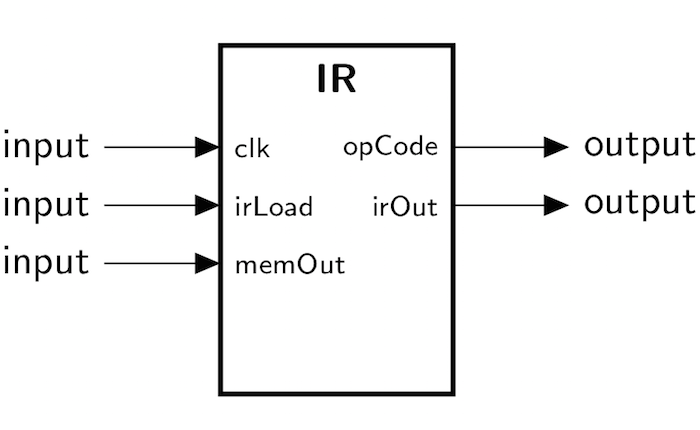
\includegraphics[width=0.4\linewidth]{images/IR.png}\\
    \captionof{figure}[Instruction Register - Block]{Instruction Register - Block}
    \label{fig:ir_block}
\end{minipage}

Das Instruction Register splittet den aktuellen Speicherwert (memOut) in einen Befehlscode (opCode) und eine Adresse (irOut).

Das Instruction Register aktualisiert diese Werte nur bei steigender Taktflanke und aktivem irLoad Signal.

\subsubsection{Ports}

\vspace{1em}
\begin{table}[!h]
	\centering
	\begin{tabular}{|l|l|c|l|}
		\hline
		\textbf{Name} & \textbf{Type} & \textbf{Bitlength} & \textbf{Direction}\\
		\hline
		clk & \texttt{std\_logic} & 1 & Input \\
		\hline
		irLoad & \texttt{std\_logic} & 1 & Input \\
		\hline
		memOut & \texttt{std\_logic\_vector} & 8 & Input \\
		\hline
		opCode & \texttt{std\_logic\_vector} & 3 & Output \\
		\hline
		irOut & \texttt{std\_logic\_vector} & 5 & Output \\
		\hline
	\end{tabular}
	\caption{Instruction Register Ports}
	\label{tab:ir_ports}
\end{table}

% ----------------------------------------------------------------------------------------------------------
% Memory Unit
% ----------------------------------------------------------------------------------------------------------

\pagebreak
\subsection{Memory Unit}

\vspace{1em}
\begin{minipage}{\linewidth}
    \centering
    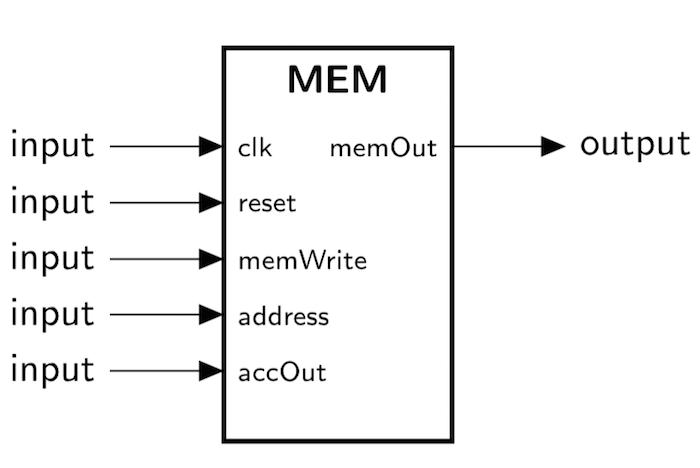
\includegraphics[width=0.4\linewidth]{images/MEM.png}\\
    \captionof{figure}[Memory Unit - Block]{Memory Unit - Block}
    \label{fig:mem_block}
\end{minipage}

Die Memory Unit stellt den Hauptspeicher des Rechners. Dieser ist 32 Byte groß. Der Speicher wird sowohl für Programmcode als auch für gespeicherte Daten verwendet.

\textbf{Funktionsweise:}

Das address Eingangssignal setzt die aktuell ausgewählte Speicherstelle. Der dort gespeicherte Wert liegt danach am Ausgangsbus memOut an.
Falls der Eingang memWrite gesetzt ist wird der Akkumulatorwert accOut in die gewählte Speicheradresse geschrieben.

Alle Daten werden erst bei einer steigenden Taktflanke.

\textbf{Reset:}

Über das reset Signal kann der Hauptspeicher zurückgesetzt werden. Hierbei werden normalerweise alle Speicherstellen auf 0 gesetzt.

Zum Testen des Rechners kann hier jedoch auch ein Programm in den Speicher geladen werden.

\subsubsection{Ports}

\vspace{1em}
\begin{table}[!h]
	\centering
	\begin{tabular}{|l|l|c|l|}
		\hline
		\textbf{Name} & \textbf{Type} & \textbf{Bitlength} & \textbf{Direction}\\
		\hline
		clk & \texttt{std\_logic} & 1 & Input \\
		\hline
	\end{tabular}
	\caption{Memory Unit Ports}
	\label{tab:mem_ports}
\end{table}

% ----------------------------------------------------------------------------------------------------------
% Program Counter
% ----------------------------------------------------------------------------------------------------------

\pagebreak
\subsection{Program Counter}

\vspace{1em}
\begin{minipage}{\linewidth}
    \centering
    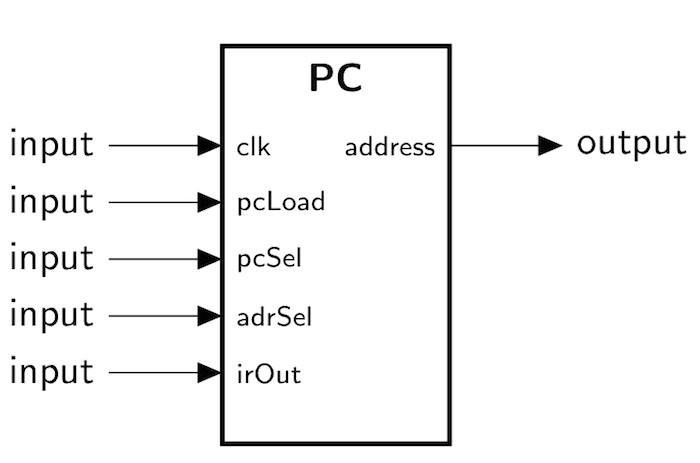
\includegraphics[width=0.4\linewidth]{images/PC.png}\\
    \captionof{figure}[Program Counter - Block]{Program Counter - Block}
    \label{fig:pc_block}
\end{minipage}

Der Program Counter hält die aktuelle Speicheradressennummer. Des weiteren erhöht er diese nach bearbeiten jedes Befehls. Er kann zudem für Sprunganweisungen und das Laden von Daten direkt auf einen Wert gesetzt werden.

\subsubsection{Ports}

\vspace{1em}
\begin{table}[!h]
	\centering
	\begin{tabular}{|l|l|c|l|}
		\hline
		\textbf{Name} & \textbf{Type} & \textbf{Bitlength} & \textbf{Direction}\\
		\hline
		clk & \texttt{std\_logic} & 1 & Input \\
		\hline
	\end{tabular}
	\caption{Program Counter Ports}
	\label{tab:pc_ports}
\end{table}

% ----------------------------------------------------------------------------------------------------------
% Central Processing Unit
% ----------------------------------------------------------------------------------------------------------

\pagebreak
\subsection{Central Processing Unit}

\vspace{1em}
\begin{minipage}{\linewidth}
    \centering
    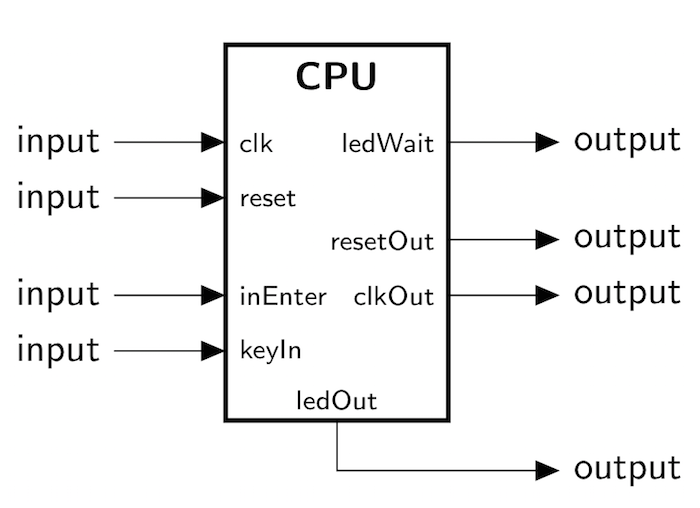
\includegraphics[width=0.4\linewidth]{images/CPU.png}\\
    \captionof{figure}[Central Processing Unit - Block]{Central Processing Unit - Block}
    \label{fig:cpu_block}
\end{minipage}

Diese VHDL Entität dient zur Verbindung der anderen Bausteine mittels dem sogenannten \emph{mapping}.

\subsubsection{Ports}

\vspace{1em}
\begin{table}[!h]
	\centering
	\begin{tabular}{|l|l|c|l|}
		\hline
		\textbf{Name} & \textbf{Type} & \textbf{Bitlength} & \textbf{Direction}\\
		\hline
		clk & \texttt{std\_logic} & 1 & Input \\
		\hline
	\end{tabular}
	\caption{Central Processing Unit Ports}
	\label{tab:cpu_ports}
\end{table}

\subsubsection{Mapping}

% ----------------------------------------------------------------------------------------------------------
% Cyclone II Pin Mapping - HC1
% ----------------------------------------------------------------------------------------------------------

\pagebreak
\subsection{Cyclone II Pin Mapping - HC1}

Um nun die HC1 CPU mit dem Quartus Board zu benutzen, müssen die Pins des Boards mit den Ein- und Ausgängen der CPU Entität verbunden werden. Dies geschieht mittels einer Top Level Entität.